\section{Derivation of the time dilation formula within VAM}\label{sec:appendix:1}

Within the Vortex Æther Model (VAM), time dilation does not arise from spacetime curvature, but from local energetic properties of the æther field, such as rotation (vorticity), pressure gradients, and topological properties of vortex structures. The local clock frequency of a vortex—associated with an elementary particle or a macroscopic object—depends on both the internal core rotation and external environmental influences such as gravitational fields and frame-dragging.

The time dilation factor $\frac{d\tau}{dt}$ is expressed in VAM as a composite correction to the universal time $t$, in which the local "own clock" $\tau$ ticks slower under the influence of:

1. Deformation of æther flow around a vortex core;
2. External gravitational vorticity caused by mass;
3. Rotating background fields.

We derive the following formula:

\begin{equation}
  \frac{d\tau}{dt} = \sqrt{1 - \frac{C_e^2}{c^2} e^{-r/r_c} - \frac{2G_\text{swirl} M_\text{eff}(r)}{r c^2} - \beta \Omega^2}
\end{equation}

Each term represents a physical mechanism:

\begin{itemize}
  \item \textbf{Term 1: Core rotation (local swirl)}
  \[
    \frac{C_e^2}{c^2} e^{-r/r_c}
  \]
  This term is derived from the intrinsic angular velocity $\Omega_\text{core}$ of the vortex core. The tangential velocity $C_e$ is the maximum swirl at the core boundary, and $r_c$ is the radius of the vortex core. The exponential factor $e^{-r/r_c}$ represents the decrease in influence at distance $r$ outside the core. This term represents the time delay due to local æther rotation.

  \item \textbf{Term 2: Gravitational field (vorticity-induced potential)}
  \[
    \frac{2 G_\text{swirl} M_\text{eff}(r)}{r c^2}
  \]
  This term mimics the classical gravitational redshift, but with an alternative gravitational constant $G_\text{swirl}$ that follows from æther parameters such as density and swirl force. The effective mass $M_\text{eff}(r)$ can be taken here as the æther vortex energy within radius $r$, instead of conventional mass. This term arises from the pressure deficit due to external swirl and replaces Newtonian gravity.

  \item \textbf{Term 3: Macroscopic rotation (frame-dragging)}
  \[
    \beta \Omega^2
  \]
  This term represents frame-dragging effects within a rotating vortex configuration (similar to the Kerr metric effect in GR). The factor $\Omega$ is the rotation rate of the macroscopic object (e.g. planet or neutron star), and $\beta$ is a coupling constant that depends on æther parameters. This term causes additional local time delay due to circulation of the surrounding æther field.

\end{itemize}

\begin{figure}[H]
  \centering
  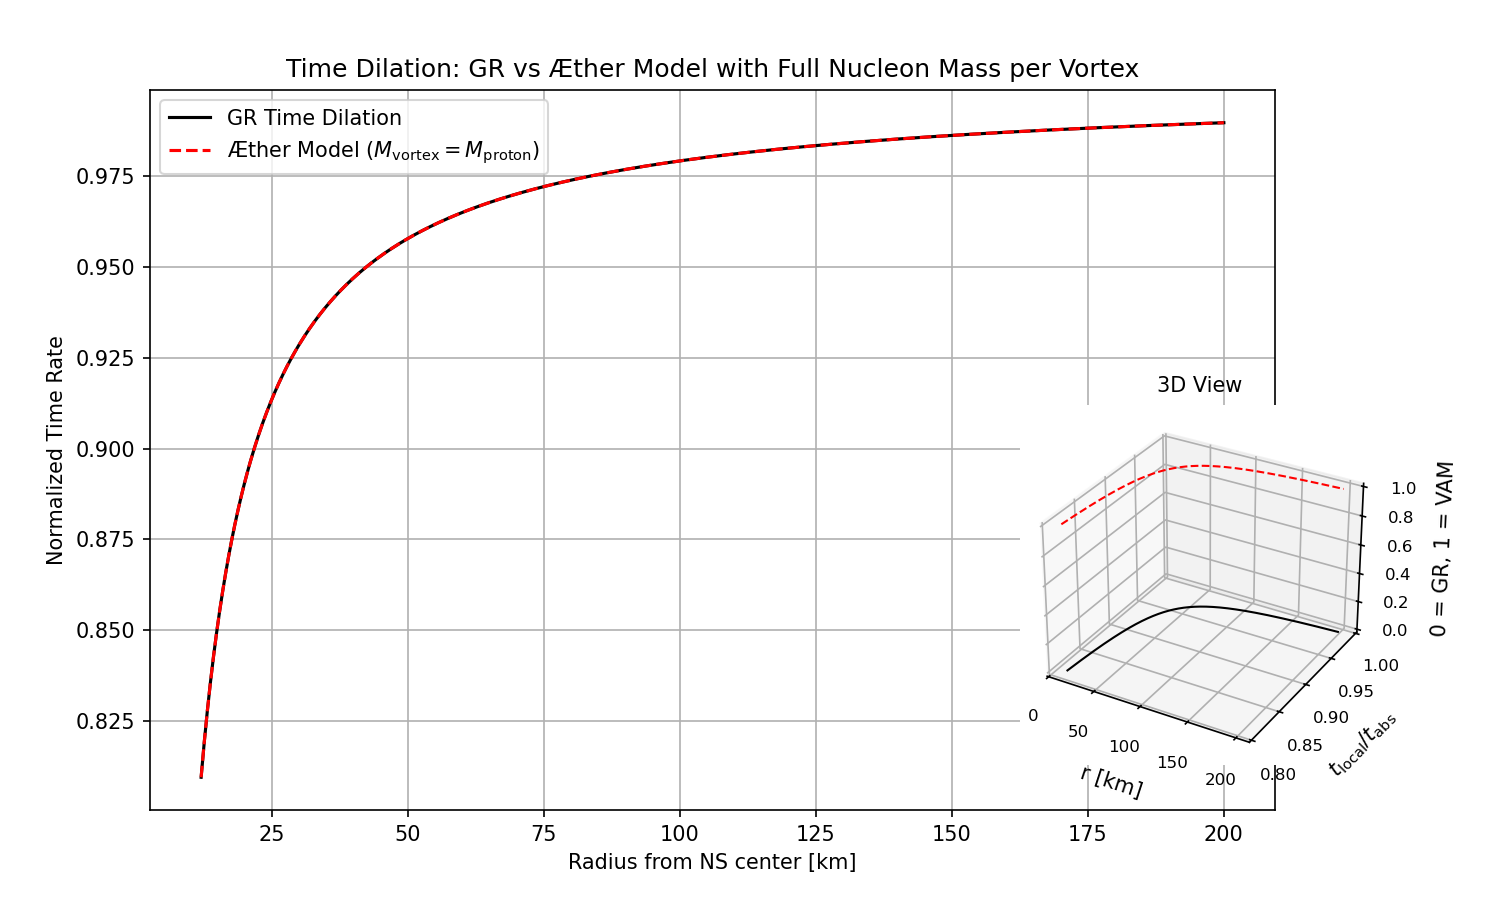
\includegraphics[width=0.85\textwidth]{images/07-TimeDilationGRVsVAM}
  \caption{
  \textbf{Comparison of Time Dilation Models:} The General Relativity (GR) time dilation formula \(\sqrt{1 - 2GM/(rc^2)}\) is contrasted with the VAM formula derived in Eq. (A1), which incorporates localized vortex angular velocity decay, vorticity-induced gravitational effects, and rotational frame dragging. The curves diverge as local rotation becomes dominant, highlighting differences in high-density regimes or vortex-based systems.
  }
  \label{fig:GRvsVAMTimeDilation}
\end{figure}



The above equation is analogous to relativistic formulas, but has a fluid mechanics origin. Experimentally, components of this formula can be found in time dilation of GPS clocks (gravity), Lense-Thirring effects (rotation), and hypothetical laboratory measurements of nuclear rotations on the quantum or vortex scale.